%%%%%%%%%%%%%%%%%%%%%%%%%%%%%%%%%%%%%%%%%%%%%%%%%%%%%%%%%%%%%%%%%%%%%%%%%%%%%%%%
%                                                                              %
% aqueous                                                                      %
%                                                                              %
%%%%%%%%%%%%%%%%%%%%%%%%%%%%%%%%%%%%%%%%%%%%%%%%%%%%%%%%%%%%%%%%%%%%%%%%%%%%%%%%
%                                                                              %
% version: 2017-05-08T1839Z                                                    %
%                                                                              %
%%%%%%%%%%%%%%%%%%%%%%%%%%%%%%%%%%%%%%%%%%%%%%%%%%%%%%%%%%%%%%%%%%%%%%%%%%%%%%%%
%                                                                              %
% LICENCE INFORMATION                                                          %
%                                                                              %
% This program produces LaTeX documents.                                       %
%                                                                              %
% copyright (C) 2013 William Breaden Madden                                    %
%                                                                              %
% This software is released under the terms of the GNU General Public License  %
% version 3 (GPLv3).                                                           %
%                                                                              %
% This program is free software: you can redistribute it and/or modify it      %
% under the terms of the GNU General Public License as published by the Free   %
% Software Foundation, either version 3 of the License, or (at your option)    %
% any later version.                                                           %
%                                                                              %
% This program is distributed in the hope that it will be useful, but WITHOUT  %
% ANY WARRANTY; without even the implied warranty of MERCHANTABILITY or        %
% FITNESS FOR A PARTICULAR PURPOSE. See the GNU General Public License for     %
% more details.                                                                %
%                                                                              %
% For a copy of the GNU General Public License, see                            %
% <http://www.gnu.org/licenses/>.                                              %
%                                                                              %
%%%%%%%%%%%%%%%%%%%%%%%%%%%%%%%%%%%%%%%%%%%%%%%%%%%%%%%%%%%%%%%%%%%%%%%%%%%%%%%%

\documentclass[american, a4paper]{report}

%%%%%%%%%%%%%%%%%%%%%%%%%%%%%%%%%%%%%%%%%%%%%%%%%%%%%%%%%%%%%%%%%%%%%%%%%%%%%%%%
%                                                                              %
% CONFIGURATION                                                                %
%                                                                              %
% - titles style                                                               %
%     - capitalisation: 0                                                      %
%     - lowercase:      1                                                      %
%     - uppercase       2                                                      %
%                                                                              %
%%%%%%%%%%%%%%%%%%%%%%%%%%%%%%%%%%%%%%%%%%%%%%%%%%%%%%%%%%%%%%%%%%%%%%%%%%%%%%%%

%%%%%%%%%%%%%%%%%%%%%%%%%%%%%%%%%%%%%%%%%%%%%%%%%%%%%%%%%%%%%%%%%%%%%%%%%%%%%%%%
% style settings                                                               %
%%%%%%%%%%%%%%%%%%%%%%%%%%%%%%%%%%%%%%%%%%%%%%%%%%%%%%%%%%%%%%%%%%%%%%%%%%%%%%%%

\edef\styleTitles{0}
\edef\demoMedia{0} % turn placeholder images on with 1 and off with 0

%%%%%%%%%%%%%%%%%%%%%%%%%%%%%%%%%%%%%%%%%%%%%%%%%%%%%%%%%%%%%%%%%%%%%%%%%%%%%%%%
% measures specifications                                                      %
%%%%%%%%%%%%%%%%%%%%%%%%%%%%%%%%%%%%%%%%%%%%%%%%%%%%%%%%%%%%%%%%%%%%%%%%%%%%%%%%

\newcommand{\measureJSpecification}{1 cm}
\newcommand{\measureKSpecification}{2 cm}
\newcommand{\measureLSpecification}{3 cm}
\newcommand{\measureMSpecification}{4 cm}
\newcommand{\measureNSpecification}{5.5 cm}
\newcommand{\measureOSpecification}{5 cm}
\newcommand{\measurePSpecification}{6 cm}
\newcommand{\measureQSpecification}{7 cm}
\newcommand{\measureRSpecification}{8 cm}
\newcommand{\measureSSpecification}{9 cm}
\newcommand{\measureTSpecification}{10 cm}
\newcommand{\measureUSpecification}{11 cm}

\usepackage{xspace}

% figure size specifications
\newcommand{\measureAFigureSpecification}{10 cm}
\newcommand{\measureBFigureSpecification}{\textwidth}
\newcommand{\measureBBFigureSpecification}{0.75\textwidth}
\newcommand{\measureCFigureSpecification}{0.5\textwidth}

% quick physics and statistics terms for use in normal text
\newcommand{\threesigma}{${3\sigma}$\xspace}
\newcommand{\fivesigma}{${5\sigma}$\xspace}
\newcommand{\ttH}{${t\bar{t}H}$\xspace}
\newcommand{\ttbar}{${t\bar{t}}$\xspace}
\newcommand{\Hbb}{${H\to bb}$\xspace}
\newcommand{\ttHbb}{${t\bar{t}H\left(b\bar{b}\right)}$\xspace}
\newcommand{\ttbb}{${t\bar{t}b\bar{b}}$\xspace}
\newcommand{\boldttHbb}{${\boldsymbol{t\bar{t}H\left(b\bar{b}\right)}}$\xspace}
\newcommand{\boldt}{${\boldsymbol{t}}$\xspace}
\newcommand{\pT}{${p_{\textrm{T}}}$\xspace}
\newcommand{\MET}{${\cancel{E}_{\textrm{T}}}$\xspace}
\newcommand{\METMM}{\cancel{E}_{\textrm{T}}\xspace} % math mode
\newcommand{\etaphi}{${\eta}$--${\phi}$\xspace}
\newcommand{\rphi}{${r}$--${\phi}$\xspace}

% silly collaboration symbols
\usepackage{stackengine}[2013-09-11]
\newcommand{\slashzero}{\stackinset{c}{}{c}{}{/}{0}\xspace}

% SM in math mode
\newcommand{\SUthreeMM}{\mathrm{SU}\left(3\right)_{\mathrm{C}}\xspace}
\newcommand{\SUtwoMM}{\mathrm{SU}\left(2\right)_{\mathrm{L}}\xspace}
\newcommand{\UoneMM}{\mathrm{U}\left(1\right)_{\mathrm{Y}}\xspace}
\newcommand{\SUfiveMM}{\textrm{SU}\left(5\right)\xspace}
\newcommand{\SUthreeSUtwoUoneMM}{\mathrm{SU}\left(3\right)_{\mathrm{C}}\times \mathrm{SU}\left(2\right)_{\mathrm{L}}\times\mathrm{U}\left(1\right)_{\mathrm{Y}}\xspace}

% SM for use in normal text
\newcommand{\SUthree}{${\SUthreeMM}$\xspace}
\newcommand{\SUtwo}{${\SUtwoMM}$\xspace}
\newcommand{\Uone}{${\UoneMM}$\xspace}
\newcommand{\SUfive}{${\SUfiveMM}$\xspace}
\newcommand{\SUthreeSUtwoUone}{${\SUthreeSUtwoUoneMM}$\xspace}

% eV units kerning
\newcommand{\eV}{\text{e\kern-0.15ex V}\xspace}
\newcommand{\MeV}{\text{M\eV}\xspace}
\newcommand{\GeV}{\text{G\eV}\xspace}
\newcommand{\TeV}{\text{T\kern-0.1ex \eV}\xspace}

% other
\newcommand{\dzero}{D\slashzero\xspace\xspace}

% software
\newcommand{\ROOT}{\textsc{ROOT}\xspace}
\newcommand{\Athena}{\textsc{Athena}\xspace}
\newcommand{\AthenaMP}{\textsc{AthenaMP}\xspace}
\newcommand{\AthenaMT}{\textsc{AthenaMT}\xspace}
%\newcommand{\ATLASJobTransforms}{\mbox{\textsc{ATLAS Job Transforms}}\xspace}
\newcommand{\ATLASJobTransforms}{\mbox{ATLAS Job Transforms}\xspace}
\newcommand{\Geant}{\textsc{Geant4}\xspace}
\newcommand{\TensorFlow}{\textsc{TensorFlow}\xspace}
\newcommand{\Keras}{\textsc{Keras}\xspace}
\newcommand{\TTHSemileptonic}{\textsc{TTHSemileptonic}\xspace}
\newcommand{\TTHbbLeptonic}{\textsc{TTHbbLeptonic}\xspace}
\newcommand{\TTHbbAnalysis}{\textsc{TTHbbAnalysis}\xspace}
\newcommand{\AnalysisBase}{\textsc{AnalysisBase}\xspace}
\newcommand{\RootCore}{\textsc{RootCore}\xspace}
\newcommand{\EventLoop}{\textsc{EventLoop}\xspace}
\newcommand{\AnalysisTop}{\textsc{AnalysisTop}\xspace}
\newcommand{\TRExFitter}{\textsc{TRExFitter}\xspace}
\newcommand{\RooFit}{\textsc{RooFit}\xspace}
\newcommand{\RooStats}{\textsc{RooStats}\xspace}
\newcommand{\Docker}{\textsc{Docker}\xspace}

% placeholder text
\newcommand{\placeholder}{
\begin{center}
\huge PLACEHOLDER
\end{center}
}
\newcommand{\placeholderfill}{
\vspace*{\fill}
\begin{center}
\huge PLACEHOLDER
\end{center}
\vspace*{\fill}
}

% epigraph, quotations
%\newcommand{\epigraph}[2]{
%    \hfill
%    \parbox{0.85\textwidth}{\em #1}\\
%    [5pt]
%    \rightline{{\rm -- #2}}
%}
\usepackage{epigraph}
\setlength{\epigraphwidth}{0.7\textwidth} % set quotations width
%\renewcommand{\epigraphrule}{0pt} % set epigraph line width
\newcommand{\epigraphcommand}[2]{
    \epigraph{#1\vspace{-10pt}}{\vspace{-0pt}#2}
}

% line spacing
\renewcommand{\baselinestretch}{1.55}

\usepackage{tabularx}

% force all subscripts to be the same height, regardless of superscripts
\usepackage{subdepth}

% line numbers
\usepackage{lineno}
\linenumbers

% subsubsections included in table of contents
\setcounter{tocdepth}{4}
\setcounter{secnumdepth}{4}

%%%%%%%%%%%%%%%%%%%%%%%%%%%%%%%%%%%%%%%%%%%%%%%%%%%%%%%%%%%%%%%%%%%%%%%%%%%%%%%%
% end of configuration                                                         %
%%%%%%%%%%%%%%%%%%%%%%%%%%%%%%%%%%%%%%%%%%%%%%%%%%%%%%%%%%%%%%%%%%%%%%%%%%%%%%%%


% graphics

\usepackage{graphicx}
\usepackage{pgf}
\usepackage{tikz}
\usepackage{pgfplots}
\usetikzlibrary{calc}
\usetikzlibrary{arrows, shapes}
\usetikzlibrary{arrows, automata}
\usetikzlibrary{positioning}

% figures

\usepackage{subfigure}
\usepackage{float}

% Gantt

% http://www.martin-kumm.de/tex_gantt_package.php
\usepackage{gantt}
\usepackage{pdflscape}

% mathematics
\usepackage{amsmath}
\usepackage{gensymb}

% floor and ceiling functions
% examples:
% - \ceil{x}
% - \ceil[\big]{x}
% - \ceil[\Big]{x}
% - \ceil[\bigg]{x}
% - \ceil[\Bigg]{x}
% (and similar for \floor)
\usepackage{mathtools}
\usetikzlibrary{fit, arrows, calc, positioning}
\DeclarePairedDelimiter{\ceil}{\lceil}{\rceil}
\DeclarePairedDelimiter{\floor}{\lfloor}{\rfloor}

% checklists
\usepackage{bbding}

% hyperlinks
\usepackage[hidelinks]{hyperref}

% verbatim
\usepackage{verbatim}
\usepackage{fancyvrb}

% justification
\usepackage{ragged2e}

% Lorem ipsum
\usepackage{lipsum}

% multiple columns
\usepackage{multicol}

% tables
\usepackage{multirow}

% time
% ISO date
\usepackage{babel}
% date formatting
\usepackage{datetime}
\newdateformat{timeA}{
    \THEYEAR-\twodigit{\THEMONTH}-\twodigit{\THEDAY}
}
\newdateformat{timeB}{
    \THEDAY~\monthname[\THEMONTH] \THEYEAR
}
\newdateformat{timeC}{
    \monthname[\THEMONTH] \THEYEAR
}
\newtimeformat{timeD}{%
    \twodigit{\THEHOUR}\twodigit{\THEMINUTE}\twodigit{\THESECOND}
}
\newtimeformat{timeE}{%
    \twodigit{\THEHOUR}\twodigit{\THEMINUTE}
}
\newdateformat{timeF}{
    \THEYEAR-\twodigit{\THEMONTH}-\twodigit{\THEDAY}T\timeD
}
\newdateformat{timeG}{
    \THEYEAR-\twodigit{\THEMONTH}-\twodigit{\THEDAY}T\timeE
}

% SI units (for micrometers etc.)
%\usepackage[mediumspace, mediumqspace, Grey, squaren]{SIunits}
\usepackage{siunitx}

% line numbers (for draft versions etc.).
% example: \linenumbers
\usepackage{lineno}

% coffee stains
\usetikzlibrary{arrows, shapes}
\usepackage{coffee4}
% example: \cofeDm{0.4}{0.1}{90}{1 cm}{-7 cm}

% embed
\usepackage{attachfile}

% titles
\usepackage{fancyhdr}
\usepackage{titlesec}

% figure command
\newcommand{\fig}[3][scale=1.0]{%
    \begin{figure}[!htbp]
        \centering
        \vspace{2 mm}
        \includegraphics[#1]{images/#2.eps}
        \caption{#3}
        \label{figure:#2}
    \end{figure}
}

% mathematics-compatible unit command
\newcommand{\mathunit}[2]{#1\,\si{#2}}

% indentation
%\setlength{\parindent}{0pt}
\usepackage{parskip}

% title styles
\ifcase\styleTitles
    % case 0
    \newcommand{\figureNameSpecification}{Figure}
    \newcommand{\tableNameSpecification}{Table}
    \newcommand{\contentsNameSpecification}{Contents}
    \newcommand{\chapterNameSpecification}{Chapter}
\or
    % case 1
    \newcommand{\figureNameSpecification}{figure}
    \newcommand{\tableNameSpecification}{table}
    \newcommand{\contentsNameSpecification}{contents}
    \newcommand{\chapterNameSpecification}{chapter}
    \titleformat{\chapter}{\Huge\bfseries}{\chapterNameSpecification~\thechapter}{1 em}{\Huge\bfseries}
\or
    % case 2
    \newcommand{\figureNameSpecification}{FIGURE}
    \newcommand{\tableNameSpecification}{TABLE}
    \newcommand{\contentsNameSpecification}{CONTENTS}
    \newcommand{\chapterNameSpecification}{CHAPTER}
    \titleformat{\chapter}{\Huge\bfseries}{\chapterNameSpecification~\thechapter}{1 em}{\Huge\bfseries}
\fi
\renewcommand{\figurename}{\figureNameSpecification}
\renewcommand{\tablename}{\tableNameSpecification}
\renewcommand{\contentsname}{\contentsNameSpecification}
\renewcommand{\chaptername}{\chapterNameSpecification}

\begin{document}

%\linenumbers

\pagenumbering{roman}

% title page
    \thispagestyle{empty}
    \begin{center}
        
\includegraphics[height=3 cm]{images/ExperPartPhys_blue.eps}
        \vspace{3.0 cm}\\
        {\large
        PROGRESS REPORT\\
        \mbox{}\\PROJECT AQUEOUS}\\
        \vspace{1.0 cm}
        \mbox{}\\
        Number 6\\
        \vspace{\fill}
        \vspace{2.0 cm}
        \vspace{\fill}
        School of Physics and Astronomy\\
        University of Glasgow\\
        \vspace{\fill}
        \timeC\today
    \end{center}

\addcontentsline{toc}{chapter}{a title for abstract}
\begin{center}
\textbf{\large a title for abstract}
\end{center}

A brief summary of the report.

\chapter*{\vspace{-80pt}\centering \large Acknowledgements \vspace{-35pt}}%
\addcontentsline{toc}{chapter}{Acknowledgements}
%\begin{comment}

The contributions of Number 2 and Number 1 are acknowledged.


% title style
\renewcommand*\contentsname{\contentsNameSpecification}
\renewcommand{\figurename}{\figureNameSpecification}
\renewcommand{\tablename}{\tableNameSpecification}

\tableofcontents

% list of figures
%\addcontentsline{toc}{chapter}{list of figures}
%\listoffigures

% list of tables
%\addcontentsline{toc}{chapter}{list of tables}
%\listoftables

\pagenumbering{arabic}

%\begin{multicols}{2}

\chapter{introduction}
\label{chapter:introduction}

\section{Higgs bosons}

Higgs bosons are particles that arise through electroweak symmetry breaking. A principal motivation for the Large Hadron Collider physics programme was the testing of the theory of electroweak symmetry breaking, through the observation of Higgs bosons. In July of 2012, the existence of the Higgs boson was confirmed by the ATLAS and CMS experiments. Following this discovery, further studies have been ongoing in order to examine the character of the particle.


\chapter{a title for chapter 1}
\label{chapter:chapter_1}
 
\section{section 1}
\label{section:section_1}

This is content.

\subsection{time}

A few time representations follow:

\begin{itemize}
\item \timeA\today
\item \timeB\today
\item \timeC\today
\item \timeD
\item \timeE
\item \timeF\today
\item \timeG\today
\end{itemize}

\subsection{units and units typesetting}

\begin{itemize}
\item \mathunit{${a^{b}}$}{m^{2}} -- correct unit typesetting (manual siunitx function) (preferred for mathematics mode, though note that the function for this is provided by aqueous [see below for manual equivalent method not dependent on aqueous])
\item \SI{10}{kg} -- correct unit typesetting (siunitx)
\item ${10\,\textnormal{kg}}$ -- incorrect unit typesetting (mathematics, textnormal)
\item 10 kg -- incorrect unit typesetting (literally)
\item \SI{10}{kg m s^{-2}} -- correct unit typesetting (siunitx)
\item ${10^{-28}}$\,\si{m^{2}} -- correct unit typesetting, though very manual (siunitx)
\item ${a^{b}}$\,\si{m^{2}} -- correct unit typesetting, though manual (siunitx) (preferred for mathematics mode)
\item \SI[parse-numbers=false]{a^{b}}{m^{2}} -- dodgy, manual correct unit typesetting (siunitx)
\item \SI[parse-numbers=false, number-math-rm=\ensuremath]{a^{b}}{m^{2}} (siunitx)
\end{itemize}

\begin{itemize}
\item The angle is ${14\degree}$.
\item The temperature is \SI{14}{\celsius}. -- correct unit typesetting (siunitx)
\end{itemize}

\subsection{mathematics}

The following is a referenced equation:

\begin{equation}
\label{equation:emc2}
E=mc^{2}
\end{equation}

This is a reference to equation \ref{equation:emc2}.

This is bold mathematics: ${t\bar{t}\bm{H}\left(b\bar{b}\right)}$.

This is bold mathematics: ${\bm{t\bar{t}H\left(b\bar{b}\right)}}$.

\subsection{lists}

This is a list:

\begin{itemize}
\item function,
\item Job,
\item JobGroup,
\item ParallelJobProcessor and
\item pool.
\end{itemize}

\newpage

This is a checklist:

\begin{description}
\item[\Checkmark] item
\item[\Checkmark] item
    \begin{description}
    \item[\Checkmark] subitem
    \item[\Checkmark] subitem
        \begin{description}
        \item[\Checkmark] subitem
        \end{description}
    \end{description}
\item[\Checkmark] item
\item[\XSolidBrush] item
\end{description}

\subsection{code}

This is some code:

\begin{center}
\footnotesize\texttt{Reco\_tf.py --inputBSFile data12.1234.RAW --outputESDFile data12.1234.ESD}
\end{center}

\subsection{images}

This is a figure set to a defined width:

\begin{figure}[H]
\begin{center}
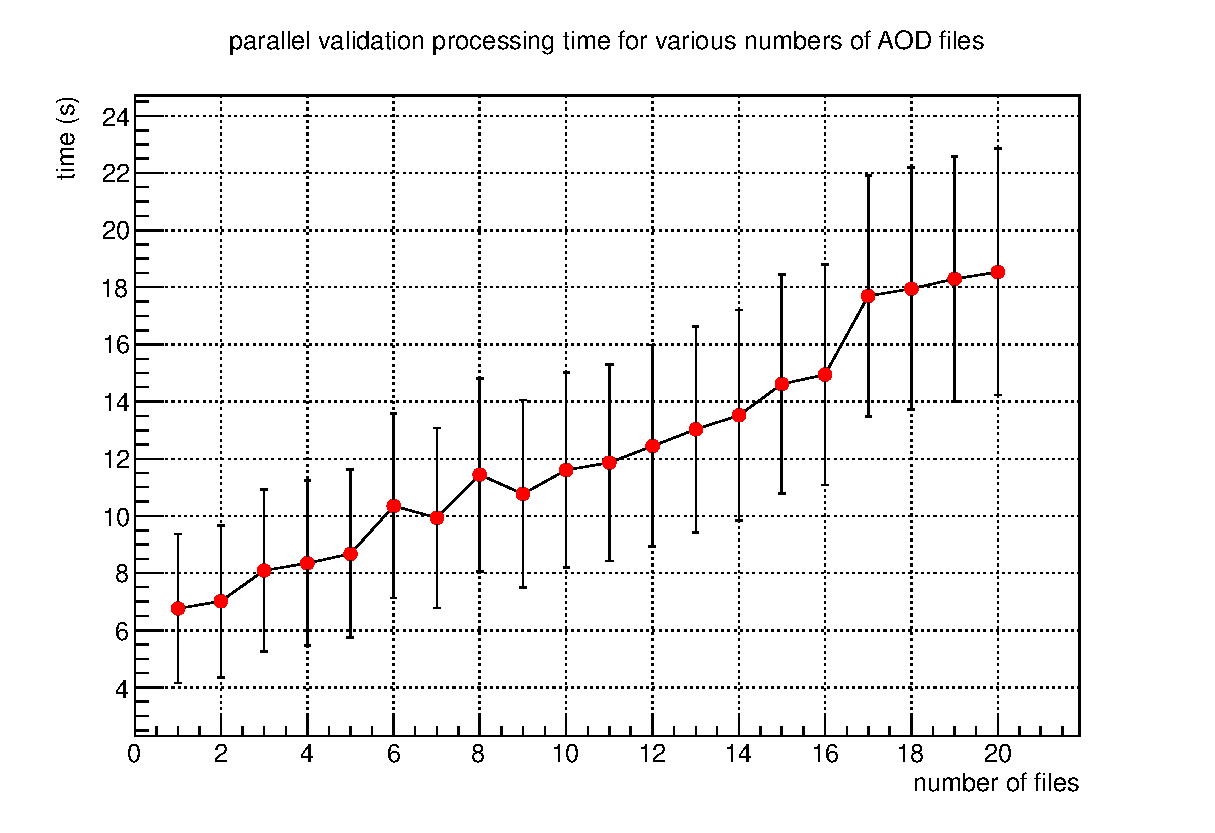
\includegraphics[width=\measureUSpecification]{images/2014-04-10_1.eps}
\end{center}
\caption{parallel job processor: large efficiency improvement as a result of parallelisation}
\end{figure}

This is a figure set to the text width:

\begin{figure}[H]
\begin{center}
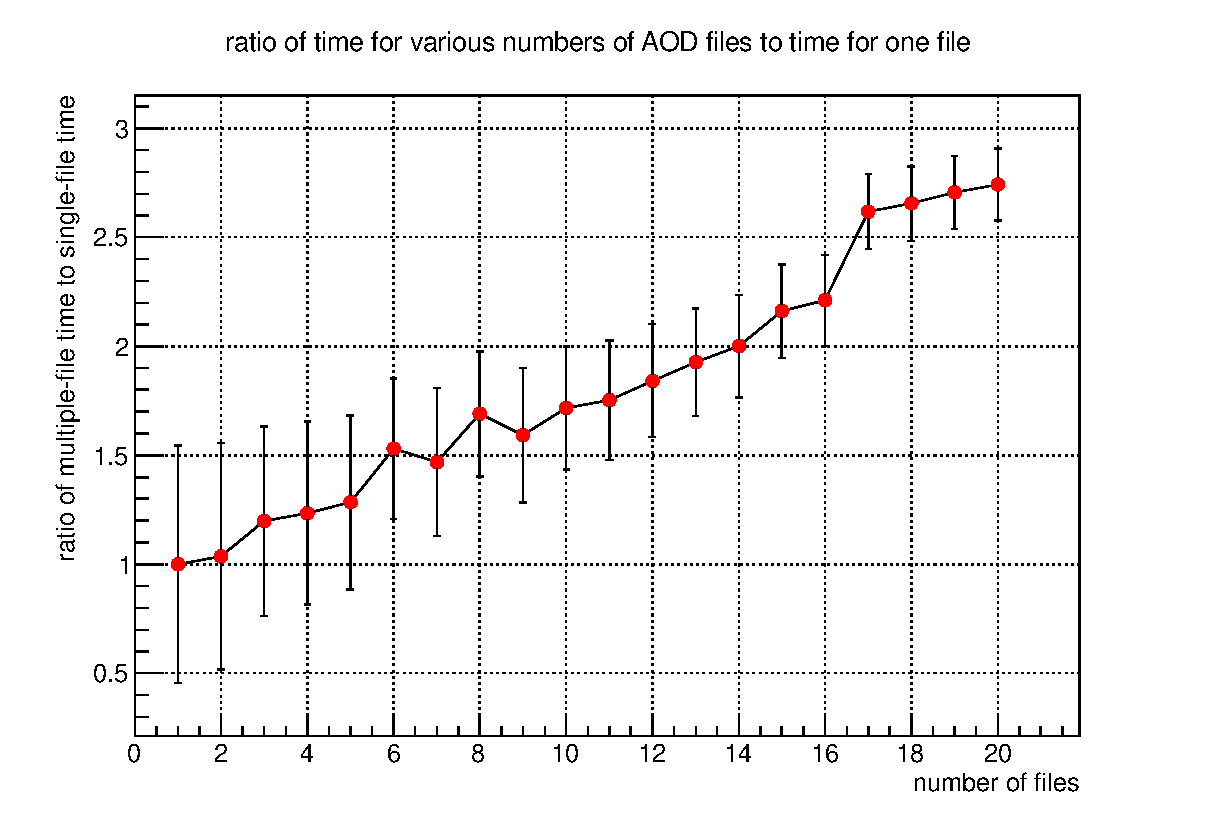
\includegraphics[width=\textwidth]{images/2014-04-10_2.eps}
\end{center}
\caption{parallel job processor}
\label{figure:PJP_1}
\end{figure}

Here is a Feynman diagram:

\begin{figure}
\begin{center}
\begin{fmffile}{gg}
\begin{fmfchar*}(50,35)

\fmfleftn{i}{2}                       % 2 initial states
\fmfrightn{o}{2}                      % 4 final states

\fmf{fermion}{i1,v1}                  % e
\fmf{fermion}{v1,i2}                  % e

\fmf{photon, label=\(\gamma\)}{v1,v2} % gamma

\fmf{fermion}{o1,v2}                  % e
\fmf{fermion}{v2,o2}                  % e

\fmflabel{\(e^{-}\)}{i1}              % gamma
\fmflabel{\(e^{-}\)}{i2}              % gamma
\fmflabel{\(e^{-}\)}{o1}              % gamma
\fmflabel{\(e^{-}\)}{o2}              % gamma

\end{fmfchar*}
\end{fmffile}
\caption{Feynman diagram}
\label{figure:Feynman_diagram_1}
\end{center}
\end{figure}

\subsection{references}

This is a reference to figure~\ref{figure:PJP_1}. This is a reference~\cite{Tianjun_1}. This is another reference~\cite{McCulloch_Pitts_1}. This is a URL: \href{https://github.com/wdbm/aqueous}{\textcolor{black!100}{https://github.com/wdbm/aqueous}}

\cofeDm{0.4}{0.1}{90}{1 cm}{-7 cm}

\subsection{ROOT}

ROOT~\cite{ROOT} is an object oriented data analysis framework aimed at solving data analysis challenges in high energy physics. While \emph{ROOT} is simply a name, a possible acronym for the system could be \emph{``Rapid Object-Oriented Technology''}~\cite{ROOT_acronym}. ROOT was developed in the context of the NA49 experiment at CERN. NA49 generated data of approximately \mathunit{10}{TB} per run. This rate of data provided a test environment for the development of ROOT, as the next generation of data analysis. ROOT features \emph{Cling}, a C++ interpreter.\footnote{This is a footnote.}

\newpage

\subsection{some paragraphs}

\lipsum[1-4]

\newpage

\subsection{tables}

\begin{figure}[h]
\begin{center}
%\begin{table}[h]
\scriptsize
\begin{tabular}{p{3 cm}p{7 cm}}
\hline\hline
input file option&description\\
\hline
\texttt{--inputHitsFile}&input only\\
\texttt{--inputBSFile}&RAW data (BS = ByteStream), currently input only\\
\texttt{--inputRDOFile}&\\
\texttt{--inputESDFile}&\\
\texttt{--inputAODFile}&\\
\hline\hline
\end{tabular}
%\end{table}
\end{center}
\mbox{}\newline
\begin{center}
%\begin{table}[h]
\scriptsize
\begin{tabular}{p{3 cm}p{7 cm}}
\hline\hline
output file option&description\\
\hline
\texttt{--outputRDOFile	valid}&if starting from Hits\\
\texttt{--outputESDFile	valid}&if starting from Hits, RDO or BS\\
\texttt{--outputAODFile	valid}&if starting from ESD or anything else upstream\\
\texttt{--outputNTUP\_XXXFile}&can be made from ESD or AOD, BS or RDO\\
\hline\hline
\end{tabular}
%\end{table}
\end{center}
\caption{Reco\_tf.py usage}
\end{figure}


\chapter{a title for future}
\label{chapter:future}

\section{future plans and considerations}

These are suggestions and plans for the future.

\begin{figure}
\label{Gantt_chart_1}
%\begin{landscape}
\begin{centering}
\scalebox{0.6}{
\begin{gantt}[
    xunitlength=0.5 cm,
    fontsize=\small,
    titlefontsize=\small,
    drawledgerline=true
]
{6}{30}
\begin{ganttitle}
    \titleelement{2015}{12}
    \titleelement{2016}{12}
    \titleelement{2017}{6}
    %\numtitle{2015}{12}{2016}{12}
\end{ganttitle}
\begin{ganttitle}
    \numtitle{1}{1}{12}{1}
    \numtitle{1}{1}{12}{1}
    \numtitle{1}{1}{6}{1}
\end{ganttitle}
\ganttbar[pattern=north west lines, color=red]{analysis 1}{0}{6}
\ganttbar[pattern=north west lines, color=blue]{analysis 2}{5}{25}
\ganttbar[pattern=north west lines, color=orange]{analysis 3}{7}{23}
\ganttbar[pattern=north west lines, color=green]{report}{24}{6}
\end{gantt}
}
%\end{landscape}
\caption{Gantt chart of work}
\end{centering}
\end{figure}

%\end{multicols}

\addcontentsline{toc}{chapter}{a title for references}
\renewcommand\bibname{a title for references}
\bibliographystyle{aqueous}
\bibliography{references}

\end{document}

